
\begin{figure}[H]
\centering
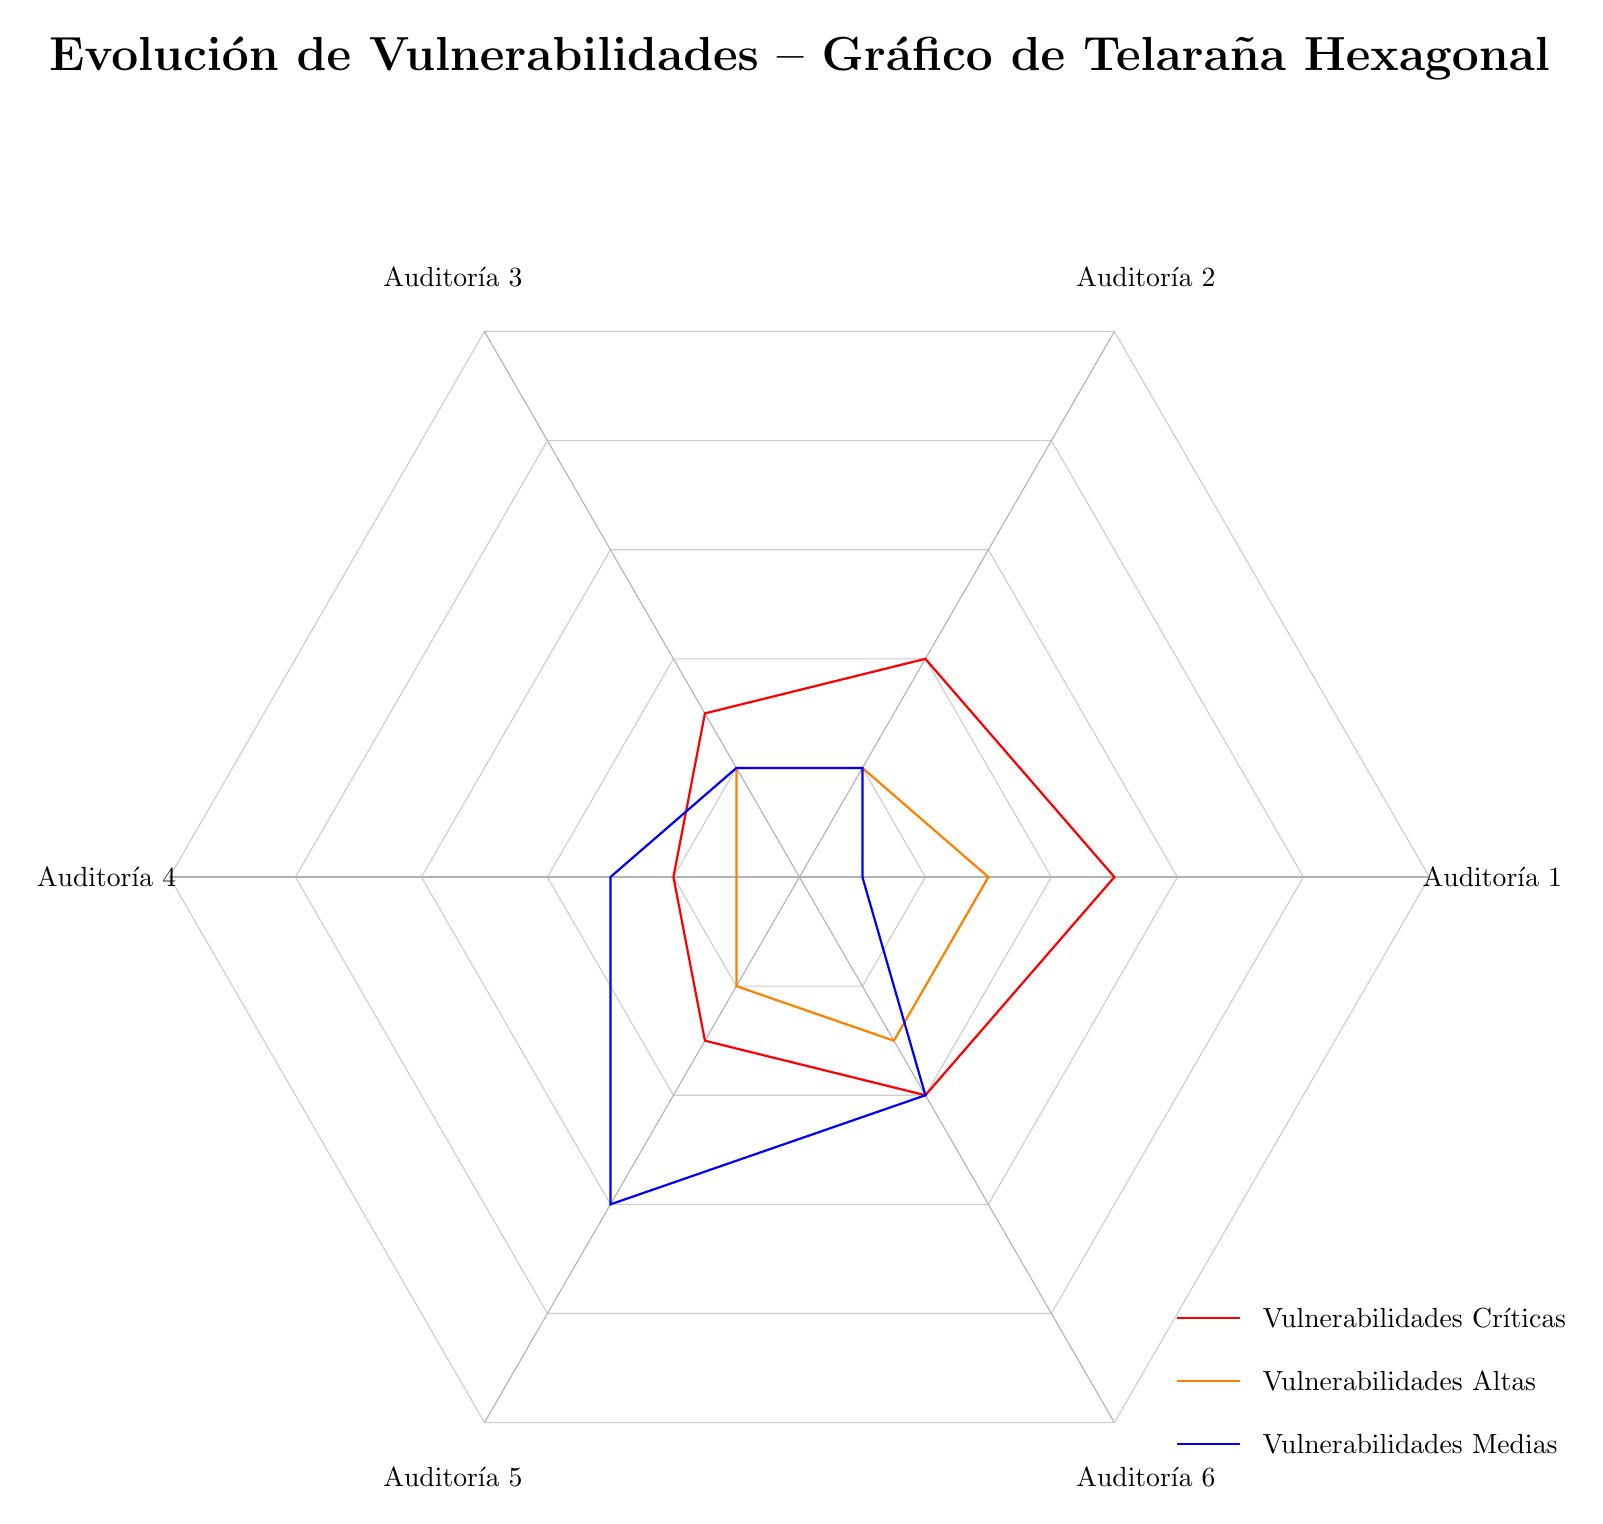
\begin{tikzpicture}[scale=0.8]

% =========================
% TELARAÑA HEXAGONAL (NIVELES)
% =========================
\foreach \r in {2,4,6,8,10} {
    \draw[gray!40] (0:\r)
        \foreach \a in {60,120,180,240,300} { -- (\a:\r) } -- cycle;
}

% =========================
% EJES RADIALES + ETIQUETAS
% =========================
\foreach \a/\label in {
    0/{Auditoría 1},
    60/{Auditoría 2},
    120/{Auditoría 3},
    180/{Auditoría 4},
    240/{Auditoría 5},
    300/{Auditoría 6}
}{
    \draw[gray!60] (0,0) -- (\a:10);
    \node at (\a:11) {\label};
}

% =========================
% SERIE: VULNERABILIDADES CRÍTICAS
% =========================
\draw[red, thick]
    (0:5) --
    (60:4) --
    (120:3) --
    (180:2) --
    (240:3) --
    (300:4) --
    cycle;

% =========================
% SERIE: VULNERABILIDADES ALTAS
% =========================
\draw[orange, thick]
    (0:3) --
    (60:2) --
    (120:2) --
    (180:1) --
    (240:2) --
    (300:3) --
    cycle;

% =========================
% SERIE: VULNERABILIDADES MEDIAS
% =========================
\draw[blue, thick]
    (0:1) --
    (60:2) --
    (120:2) --
    (180:3) --
    (240:6) --
    (300:4) --
    cycle;

% =========================
% LEYENDA
% =========================
\begin{scope}[shift={(6,-7)}]
    \draw[red, thick] (0,0) -- (1,0);
    \node[right] at (1.2,0) {Vulnerabilidades Críticas};

    \draw[orange, thick] (0,-1) -- (1,-1);
    \node[right] at (1.2,-1) {Vulnerabilidades Altas};

    \draw[blue, thick] (0,-2) -- (1,-2);
    \node[right] at (1.2,-2) {Vulnerabilidades Medias};
\end{scope}

% =========================
% TÍTULO
% =========================
\node[font=\LARGE\bfseries] at (0,13)
{Evolución de Vulnerabilidades – Gráfico de Telaraña Hexagonal};

\end{tikzpicture}
\caption{Comparación de vulnerabilidades mediante gráfico de telaraña hexagonal}
\end{figure}
